\documentclass[tikz,border=10pt]{standalone}
\usepackage{tkz-euclide}
\usetkzobj{all}
\usetikzlibrary{quotes,angles,positioning}
\begin{document}
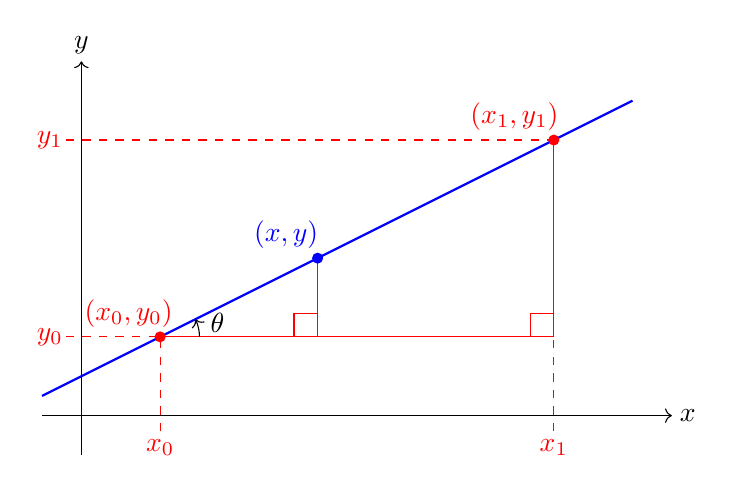
\begin{tikzpicture}
	\coordinate (A) at (6,3.5);
	\coordinate (B) at (3,2);
	\coordinate (C) at (1,1);
	\coordinate (D) at (3,1);
	\coordinate (E) at (6,1);
	\coordinate (O) at (-0.5,0.25);
	\coordinate (o1) at (1,-0.2);
	\coordinate (o3) at (3,-0.2);
	\coordinate (o6) at (6,-0.2);
	\coordinate (o8) at (7,4);
	\coordinate (oC) at (-0.2,1);
	\coordinate (oB) at (-0.2,2);
	\coordinate (oA) at (-0.2, 3.5);
	\coordinate (oX) at (7.5,0);
	\coordinate (oY) at (0,4.5);
	\coordinate (XoY) at (0,0);
	\coordinate (Yo) at (0,-0.5);
	\coordinate (Xo) at (-0.5,0);

	\draw [->](Xo)--(oX);
	\draw [->](Yo)--(oY);
	\draw [blue, thick] (O) -- (o8);
	\draw [red] (C)--(E);
	\draw [red] (D)--(B);
	\draw [red] (E)--(A);
	\draw [red,dashed] (o1)--(C);
	\draw [red,dashed] (o6)--(A);
	\draw [red,dashed] (oC)--(C);
	\draw [red,dashed] (oA)--(A);

 	\fill[red] (intersection of O--A and C--D) circle (2pt);
	\fill[red] (intersection of O--A and E--A) circle (2pt);
	\fill[blue] (intersection of O--A and B--D) circle (2pt);

	\pic [draw, ->, "$\theta$", angle eccentricity=1.5] {angle = E--C--A};
	\tkzMarkRightAngle[draw=red,size=.3](D,E,A);
	\tkzMarkRightAngle[draw=red,size=.3](C,D,B);

	\node[red] (x0y0) at (0.6,1.3) {$(x_0,y_0)$};
	\node[red] (x1y1) at (5.5,3.8) {$(x_1,y_1)$};
	\node[blue] (xnyn) at (2.6,2.3) {$(x,y)$};
	\node (xLabel) at (7.7,0) {$x$};
	\node (yLabel) at (0,4.7) {$y$};
	\node [red](x0) at (1,-0.4) {$x_0$};
	\node [red](x1) at (6,-0.4) {$x_1$};
	\node [red](y0) at (-0.4,1) {$y_0$};
	\node [red](y1) at (-0.4,3.5) {$y_1$};

\end{tikzpicture}
\end{document}